\documentclass[]{article}
\usepackage{amsmath}
\usepackage{graphicx}


\begin{document}

In this post, I will briefly review the basic theory about ordinary linear regression using frequentist and Bayesian estimation methods. This will lay the terrain for a later post about Gaussian Processes. This post closely follows the presentation in Murphy (2012).

\section{Basics of Linear Regression}

Linear regression used to fit a model that is linear in the parameters to a data set $\mathcal{D}=\{\boldsymbol{X},\boldsymbol{y}\}$, where $\boldsymbol{X}$ represents the independent variables and $\boldsymbol{y}$ the dependent variable, and has the form

$p(y|\boldsymbol{x}, \boldsymbol{\beta}) = \mathcal{N}(y|\boldsymbol{\beta}^T\boldsymbol{x}, \sigma_{\epsilon}^2)$

where $\boldsymbol{\beta}$ is a vector of model parameters and $\sigma_{\epsilon}^2$ is the model error variance. The unusual notation for the normal distribution $\mathcal{N}$ should be read as "a normal distribution of $\boldsymbol{y}$ with (or given) mean $\boldsymbol{\beta}^T\boldsymbol{x}$ and variance $\sigma_{\epsilon}^2$." The traditional method of estimating the parameters of a linear regression model is by using the frequentist method of maximum likelihood estimation (MLE). MLE provides point estimates $\boldsymbol{\hat{\beta}}$ for each of the regression model parameters $\boldsymbol{\beta}$ by maximizing the likelihood function with respect to $\boldsymbol{\beta}$ and $\sigma_{\epsilon}^2$ by solving the minimization problem

$\boldsymbol{\hat{\beta}} = arg\,\underset{\boldsymbol{\beta}}{max}\;\mathcal{L}(\boldsymbol{\beta})$

where the likelihood function $\mathcal{L}(\boldsymbol{\beta})$ is defined as

$\mathcal{L}(\boldsymbol{\beta})=p(\mathcal{D}|\boldsymbol{\beta})={\displaystyle \prod_{i=1}^{N} p(y_i|\boldsymbol{x}_i, \boldsymbol{\beta}, \mu, \sigma_{\epsilon}^2)} = \mathcal{N}(\boldsymbol{y}|\mu + \boldsymbol{X}\boldsymbol{\beta},\sigma_{\epsilon}^2\boldsymbol{I})$

where $\mu$ is the mean of the model error ($\mu=0$ hereafter), $N$ is the number of points in the data set, $\boldsymbol{I}$ is an identity matrix, and $\boldsymbol{x}$ is a vector of values of the independent variables for an individual data point of matrix $\boldsymbol{X}$. If a non-linear function shape is sought, linear regression can be used to fit a model linear in the parameters over a function $\phi(\cdot)$ of the data. This procedure is called basis function expansion and has a likelihood function of the form

$\mathcal{L}(\boldsymbol{\beta}) = \mathcal{N}(\boldsymbol{y}|\mu + \phi(\boldsymbol{X})\boldsymbol{\beta},\sigma_{\epsilon}^2\boldsymbol{I})$

where $\phi(\boldsymbol{x})$ can have, for example, the form

$\phi(\boldsymbol{x})=[1, x_1, x_1^2]$

for fitting a parabola to a one-dimensional $\boldsymbol{X}$ over $\boldsymbol{y}$. When minimizing the squared residuals we get to the famous Ordinary Least Squares regression. Linear regression can be further developed, for example, into Ridge Regression to better handle multicollinearity by introducing bias to the parameter estimates, and into Kernel Ridge regression to implicitly add non-linear terms to the model. These formulations are beyond the scope of this post.

What is important to notice is that the standard approaches for linear regression described here, although able to fit linear and non-linear functions, do not provide much insight into the model errors. That is when Bayesian methods come to play.

\section{Bayesian Linear Regression}

In Bayesian Linear regression (and in any Bayesian approach), the parameters $\boldsymbol{\beta}$ are treated themselves as random variables. This allows for the consideration of model uncertainty, given that now instead of having the best point estimates for $\boldsymbol{\beta}$ we have their full distributions from which to sample models – a sample of  $\boldsymbol{\beta}$ corresponds to a model. The distribution of parameters for $\boldsymbol{\beta}$, $P(\boldsymbol{\beta}|\mathcal{D})$, called the parameter posterior distribution, is calculated by multiplying the likelihood function used in MLE by a prior distribution for the parameters. A prior distribution is assumed from knowledge prior to analyzing new data. In Bayesian Linear Regression, a Gaussian distribution is commonly assumed for the parameters. For example, the prior on $\boldsymbol{\beta}$ can be $\mathcal{N}(\boldsymbol{\beta_0},\boldsymbol{V}_0)$ for algebraic simplicity. The parameter posterior distribution assuming a known  then has the form

$p(\boldsymbol{\beta}|\mathcal{D}, \sigma^2) =\frac{p(\mathcal{D}|\boldsymbol{\beta}, \sigma^2)p(\boldsymbol{\beta})}{p(\mathcal{D})} \propto p(\mathcal{D}|\boldsymbol{\beta}, \sigma^2)p(\boldsymbol{\beta})$  ,        given $p(\mathcal{D})$ is a constant depending only on the data.

We now have an expression from which to derive our parameter posterior for our linear model from which to sample $\boldsymbol{\beta}$. If the likelihood and the prior are Gaussian, the parameter posterior will also be a Gaussian, given by

$p(\boldsymbol{\beta}|\mathcal{D}, \sigma^2) \propto \mathcal{N}(\boldsymbol{\beta}|\boldsymbol{\beta}_0, \boldsymbol{V}_0)\mathcal{N}(\boldsymbol{y}|\boldsymbol{X\beta},\sigma^2\boldsymbol{I})=\mathcal{N}(\boldsymbol{\beta}|\boldsymbol{\beta}_N,\boldsymbol{V}_N)$
where
$\boldsymbol{V}_N = \sigma^2(\sigma^2\boldsymbol{V}_0^{-1}+\boldsymbol{X}^T\boldsymbol{X})^{-1}$
$\boldsymbol{\beta}_N=\boldsymbol{V}_N\boldsymbol{V}_0^{-1}\boldsymbol{\beta}_0 + \frac{1}{\sigma^2}\boldsymbol{V}_N\boldsymbol{X}^T\boldsymbol{y}$

If we calculate the parameter posterior (distribution over parameters $\boldsymbol{\beta}$) for a simple linear model $f(x) = \beta_0 + \beta_1x$ for a data set $\mathcal{D}$ in which $\boldsymbol{X}$ and $\boldsymbol{y}$ are approximately linearly related given some noise $\sigma_{\epsilon}^2$, we can use it to sample values for $\boldsymbol{\beta}$. This is equivalent to sampling linear models $f(x)$ for data set $\mathcal{D}$. As the number of data points increase, the variability of the sampled models should decrease, as in the figure below

\begin{figure}
	\centering
	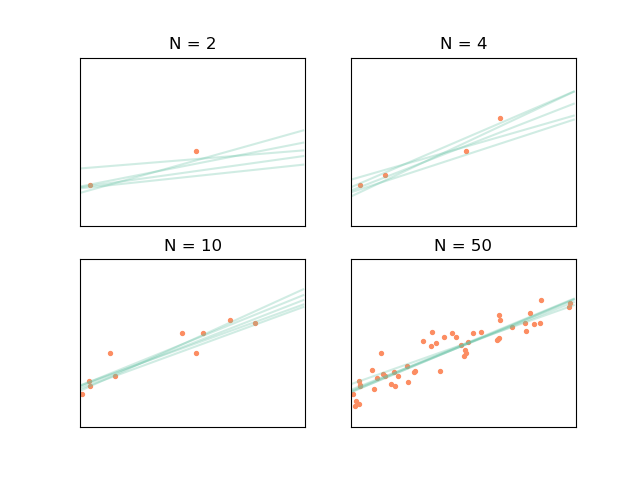
\includegraphics[width=0.9\linewidth]{linear_model.png}
	\label{fig:linearmodel}
\end{figure}

This is all interesting but the parameter posterior per se is not of much use. We can, however, use the parameter posterior to find the posterior predictive distribution, which can be used to both get point estimates of $y$ and the associated error. This is done by multiplying the likelihood by the parameter posterior and marginalizing the result over $\boldsymbol{\beta}$. This is equivalent to performing infinite sampling of blue lines in the example before to form density functions around a point estimate of $\mu_{y_*}=f(\boldsymbol{x}_*)$, with $(\boldsymbol{x}_*,y_*)$ denoting a new point that is not in $\mathcal{D}$. If the likelihood and the parameter posterior are Gaussian, the posterior predictive then takes the form below and will also be Gaussian (in Bayesian parlance, this means that the Gaussian distribution is conjugate to itself)!

$\begin{aligned}p(y_*|x_*,\mathcal{D}, \sigma_{\epsilon}^2) &= \int_{\boldsymbol{\beta}}p(y_*|x_*,\mathcal{D}, \sigma_{\epsilon}^2,\boldsymbol{\beta})p(\boldsymbol{\beta}|\mathcal{D}, \sigma)d\boldsymbol{\beta}\\

&=\mathcal{N}(\boldsymbol{\beta}_N^T, \sigma_N^2(\boldsymbol{x}_*))\end{aligned}$

where

$\sigma_N^2(\boldsymbol{x}_*) = \sigma_{\epsilon}^2 + x^{*T}\boldsymbol{V}_Nx_*$

or, to put it simply,

$\boldsymbol{y}_* = f(\boldsymbol{x}_*) = \boldsymbol{\beta}_N(\boldsymbol{x}_*) \pm \sigma_N^2(\boldsymbol{x}_*)$

The posterior predictive, meaning final linear model and associated errors (the parameter uncertainty equivalent of frequentist statistics confidence intervals) are shown below

\begin{figure}
	\centering
	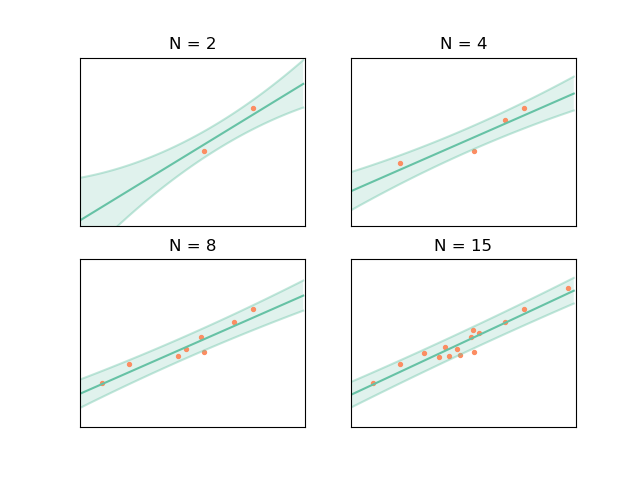
\includegraphics[width=0.9\linewidth]{linear_regression.png}
	\label{fig:linearregression}
\end{figure}

If, instead of having a data set $\mathcal{D}$ in which $\boldsymbol{X}$ and $\boldsymbol{y}$ are related approximately according to a 4th order polynomial, we use a $\phi(\cdot)$ function to artificially create more random variables (or features, in machine learning parlance) corresponding to the non-linear terms of the polynomial function. Our function $\phi(\cdot)$ would be $\phi(x) = [1, x, x^2, x^3, x^4]$ and the resulting $X$ would therefore have five columns instead of two ($[1, x]$), so now the task is to find $\boldsymbol{\beta}=[\beta_0, \beta_1, \beta_2, \beta_3, \beta_4]$. Following the same logic as before for $X'=\phi(X)$ and $x_*'=\phi(x_*)$, where prime denotes the new set random variable $x$ from function $\phi(\cdot)$, we get the following plots

\begin{figure}
	\centering
	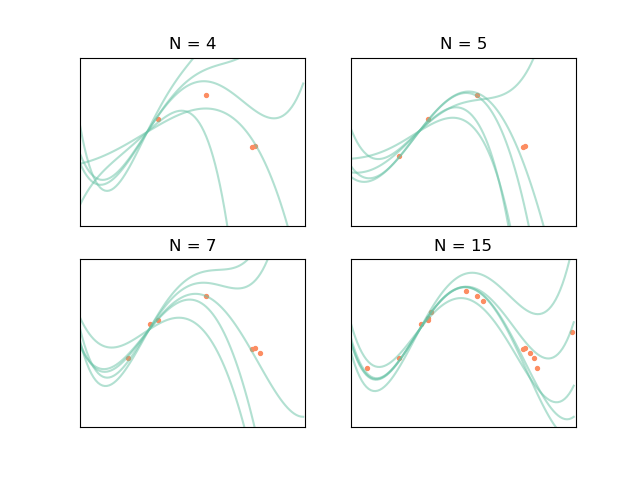
\includegraphics[width=0.9\linewidth]{poly_model.png}
	\caption{}
	\label{fig:polymodel}
\end{figure}

\begin{figure}
	\centering
	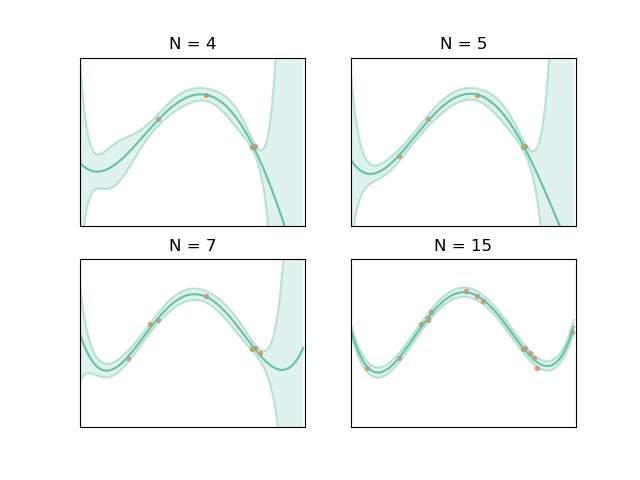
\includegraphics[width=0.9\linewidth]{poly_regression.png}
	\caption{}
	\label{fig:polyregression}
\end{figure}

This looks great, but there is a problem: what if we do not know the functional form of the model we are supposed to fit (e.g. a simple linear function or a 4th order polynomial)? This is often the case, such as when modeling the reliability of a water reservoir system contingent on stored volumes, inflows and evaporation rates, or when modeling topography based on samples surveyed points (we do not have detailed elevation information about the terrain, e.g. a DEM file). Gaussian Processes (GPs) provide a way of going around this difficulty.

\section{References}

Murphy, Kevin P., 2012. Machine Learning: A Probabilistic Perspective. The MIT Press.

\end{document}
